\documentclass[11pt,a4paper]{ctexart}
\usepackage[margin=2.05cm]{geometry}
\usepackage{amsmath,amssymb,bm}
\usepackage{booktabs,graphicx,xcolor,hyperref}
\hypersetup{colorlinks=true,linkcolor=blue,urlcolor=blue}
\setlength{\parindent}{2em}
\setlength{\parskip}{0.3em}
\title{IMU--UWB InEKF：论文--代码一致性最小修正版}
\author{仅修复明确不一致，不加入其他算法改进}
\date{2026年7月23日}

\begin{document}
\maketitle

\section{修改边界}

本版本以原始提交 \texttt{f3b664e} 为基线，只修复两项可由论文公式和代码直接证明的
不一致：偏置状态顺序，以及 $SO(3)$ 左雅可比零角分支的符号。没有加入中点积分、
严格异步传播、Van Loan 噪声离散化、静止更新、静态偏置初始化、新杠杆臂雅可比、
协方差 reset 或快速调度。

\section{偏置顺序：从相互冲突到唯一含义}

论文第~4 页式 (27)--(29) 将陀螺仪偏置和加速度计偏置依次写为
\begin{equation}
 \bm\zeta =
 \begin{bmatrix}
 \hat{\bm b}_{g}-\bm b_g\\
 \hat{\bm b}_{a}-\bm b_a
 \end{bmatrix},
 \qquad
 \delta\bm x =
 \begin{bmatrix}
 \delta\bm\theta&
 \delta\bm v&
 \delta\bm p&
 \delta\bm b_g&
 \delta\bm b_a
 \end{bmatrix}^{\mathsf T}.
 \label{eq:paper-order}
\end{equation}

原代码的名义传播却采用
\begin{equation}
 \bm b_{\mathrm{nominal}}^{\mathrm{original}}
 =
 \begin{bmatrix}\bm b_a&\bm b_g\end{bmatrix}^{\mathsf T},
\end{equation}
而传播矩阵 $A$ 的第四个三维块按 $\bm b_g$ 使用，$P_0$ 和 $Q$ 的第四块又按
$\bm b_a$ 初始化。因此相同的索引同时具有两种物理含义。

修正版统一为式~\eqref{eq:paper-order}：
\begin{align}
 \bm\omega &= \bm\omega_m-\bm b_g,
 &
 \bm a &= g\,\bm a_m-\bm b_a,\\
 P_0 &=
 \operatorname{diag}\!\left(
 P_{\theta},P_v,P_p,
 \sigma_{b_g}^2I_3,\sigma_{b_a}^2I_3
 \right),\\
 Q &=
 \operatorname{diag}\!\left(
 Q_g,Q_a,0_3,Q_{b_g},Q_{b_a}
 \right)\Delta t^2.
\end{align}
这里没有改变噪声数值、传播阶次或离散公式，只交换错误的物理块次序。

\section{\texorpdfstring{$SO(3)$}{SO(3)} 左雅可比零角符号}

论文第~3 页式 (11) 的一阶项为
\begin{equation}
 J_l(\bm\phi)
 =
 I_3+\frac{1}{2}\bm\phi^\wedge+O(\lVert\bm\phi\rVert^2).
\end{equation}
原代码的一般分支对应正号，但零角分支返回
\begin{equation}
 J_{l,\mathrm{original}}
 \approx I_3-\frac{1}{2}\bm\phi^\wedge,
\end{equation}
因而分支前后含义不连续。修正版只将负号改为正号：
\begin{equation}
 J_{l,\mathrm{fixed}}
 \approx I_3+\frac{1}{2}\bm\phi^\wedge.
\end{equation}
仍然沿用原来的一阶近似，没有换用更高阶数值公式。

\section{完整数据结果}

在完整 \texttt{const1-trial1-tdoa2.csv} 上，两种实现使用相同的原始事件语义、
初始化、噪声和外部评价器。共有 209167 个状态样本和 67205 个 UWB 测量。

\begin{table}[htbp]
\centering
\caption{原始代码与论文一致修正版的完整 const1 对比}
\begin{tabular}{lrrr}
\toprule
指标 & 原始代码 & 修正版 & 相对变化\\
\midrule
位置 RMSE (m) & 0.106713662 & 0.106715766 & $+0.00197\%$\\
速度 RMSE (m/s) & 0.059415186 & 0.059434733 & $+0.03290\%$\\
测地姿态 RMSE (rad) & 0.061042702 & 0.061136358 & $+0.15343\%$\\
yaw RMSE (rad) & 0.059456002 & 0.059550649 & $+0.15919\%$\\
UWB 拒绝数 & 0/67205 & 0/67205 & 不变\\
\bottomrule
\end{tabular}
\end{table}

四项误差均有极小幅度增加，不能声称精度改善。由于此数据以零偏置初始化、偏置随机
游走很小，偏置索引修正对轨迹的影响有限；其价值是恢复偏置、交叉协方差和后续状态
更新的正确物理含义。

为隔离偏置顺序的独立影响，另一次受控消融恢复原始左雅可比小角度分支，同时保持原始
偏置先验和随机游走数值，只统一名义偏置、$P_0$ 和 $Q$ 的
$[\bm b_g,\bm b_a]$ 顺序。所得四项 RMSE 与表中修正版一致到报告精度。因此在完整
const1 和原始极小偏置调谐下，可以将位置 $+0.001972\%$、速度 $+0.032899\%$、姿态
$+0.153427\%$、yaw $+0.159188\%$ 的变化归因于偏置顺序修正，而不是左雅可比符号。
但这一确定性数据结果不构成跨轨迹的统计结论，且幅度没有工程显著性。

\begin{figure}[htbp]
\centering
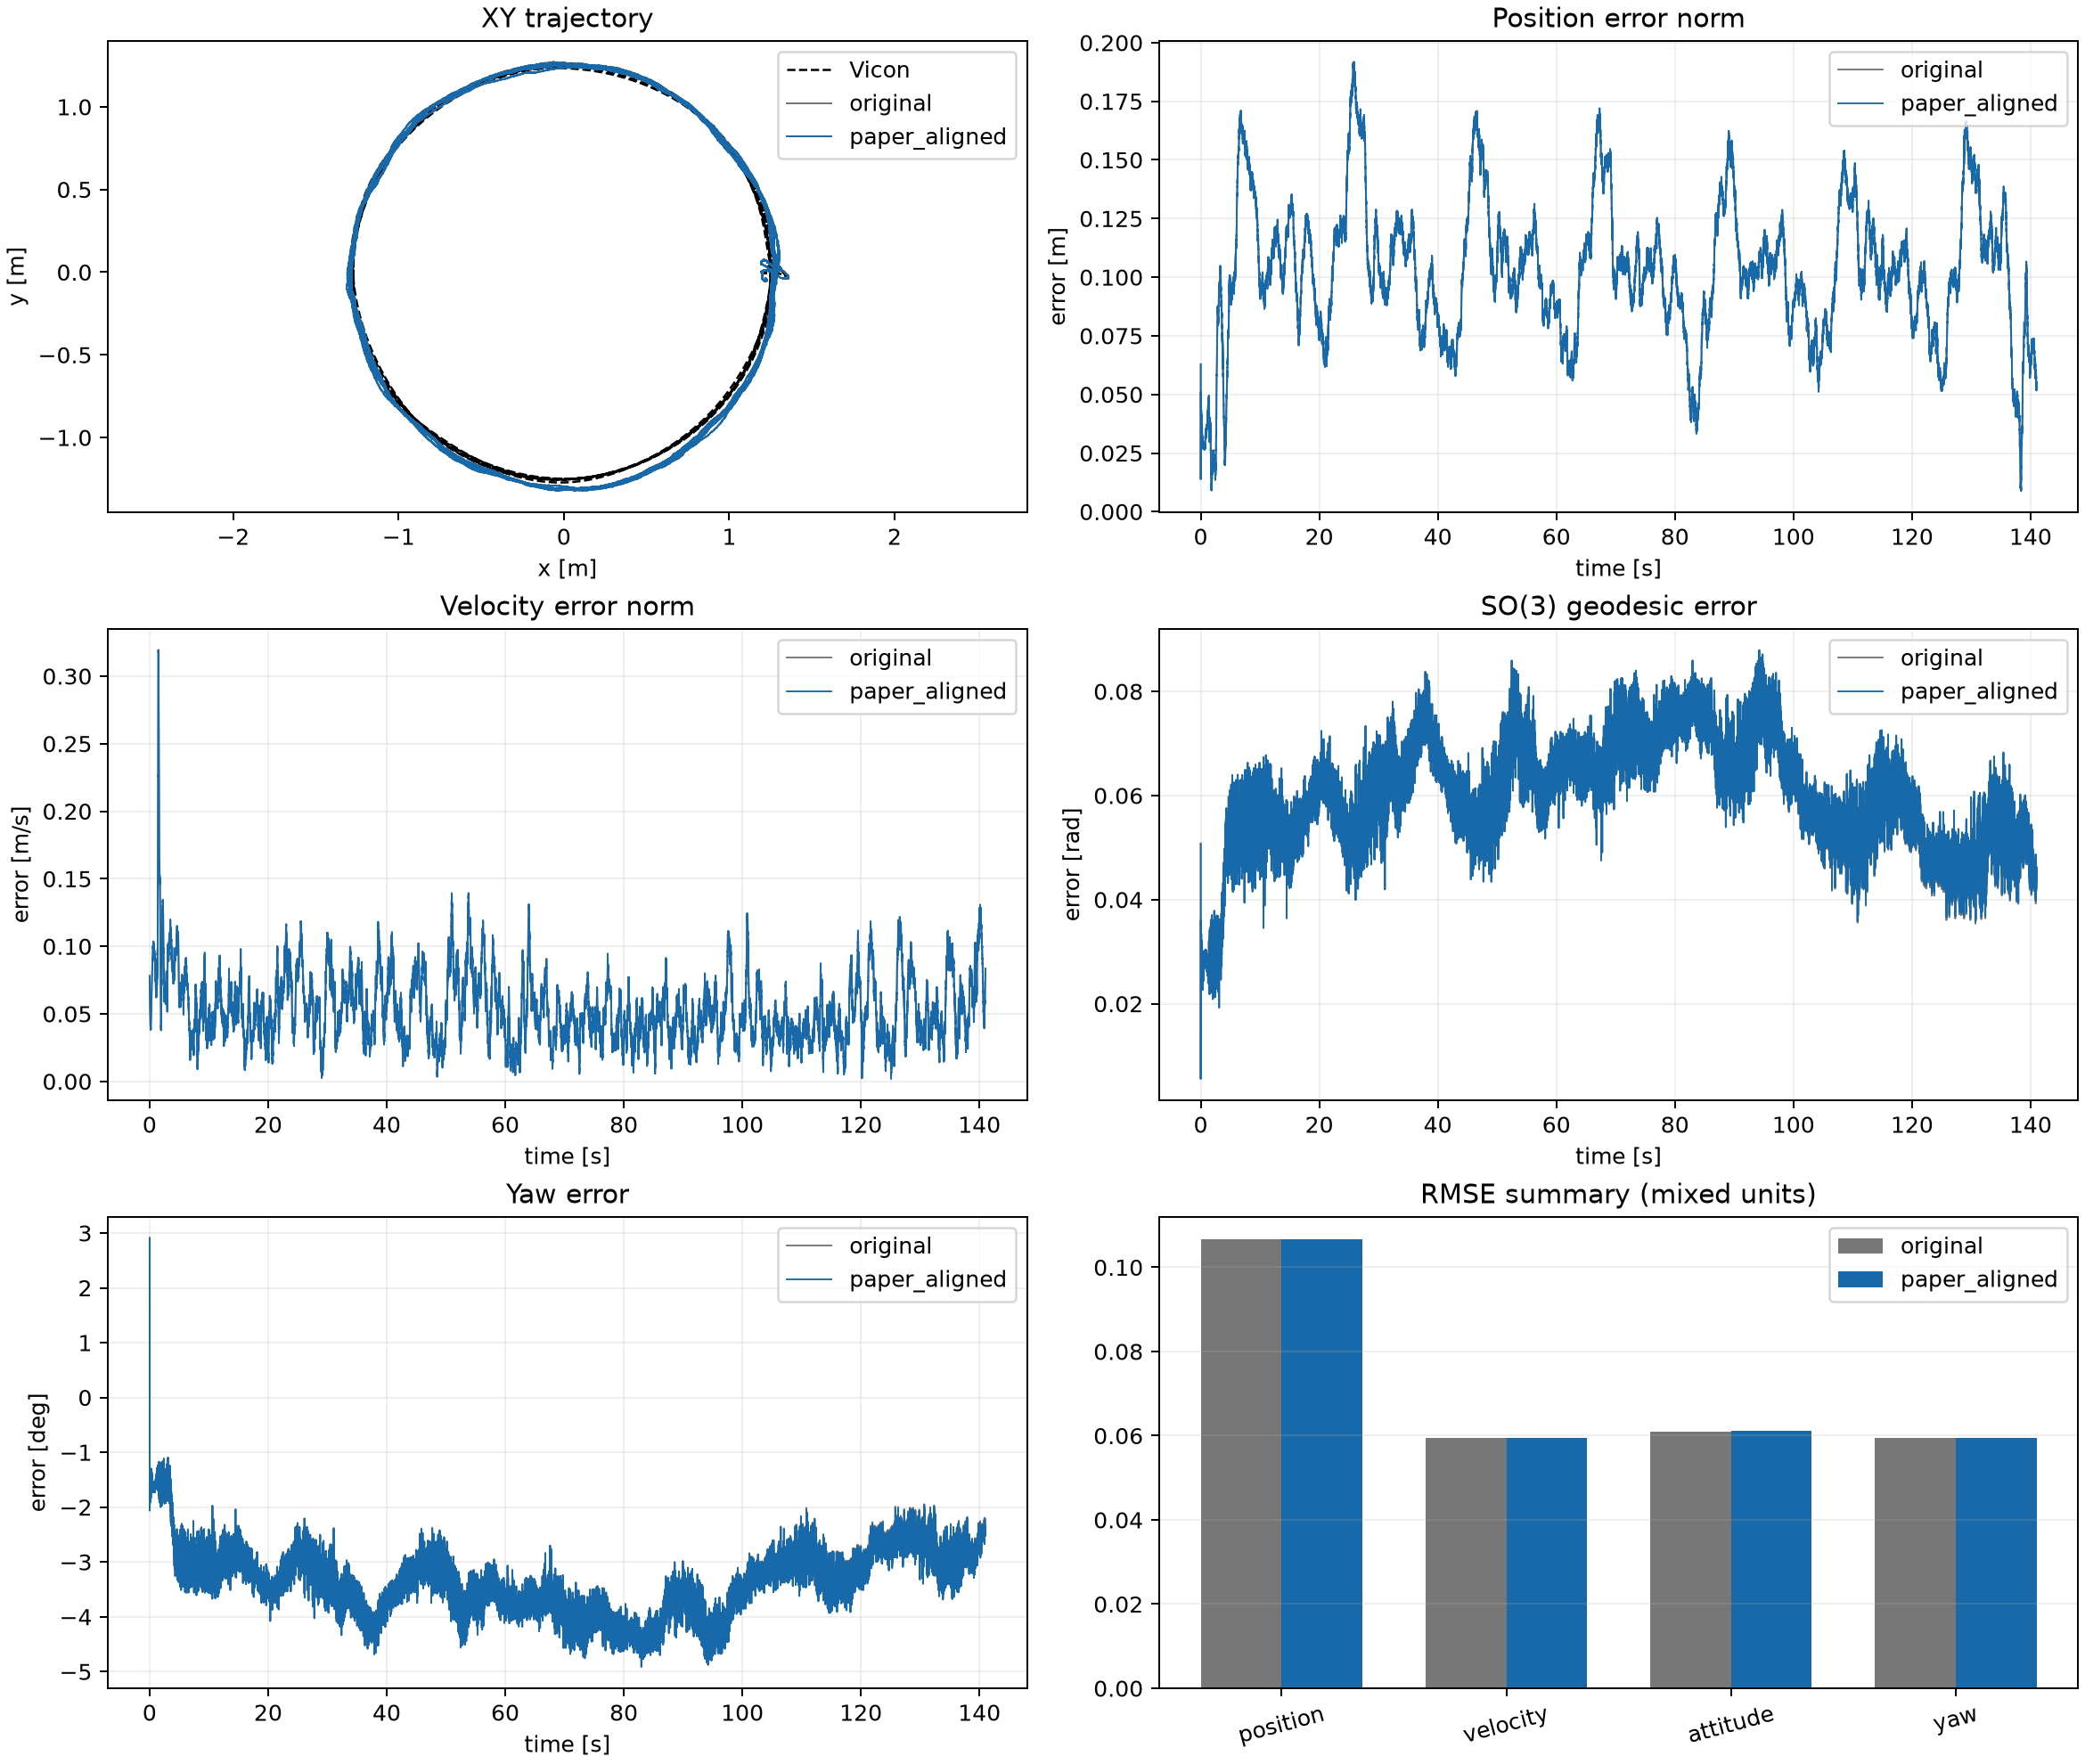
\includegraphics[width=\textwidth]{../imu-uwb-inekf-fix/results/paper_alignment_const1_full/comparison.png}
\caption{完整 const1 对比。两条曲线几乎重合，未出现新增峰值、跳变或发散。}
\end{figure}

\section{耗时与结论}

两种顺序的完整回放为：
\begin{center}
\begin{tabular}{lrr}
\toprule
顺序 & 第一次/s & 第二次/s\\
\midrule
Original$\rightarrow$Fixed & 48.280 & 36.507\\
Fixed$\rightarrow$Original & 37.453 & 40.156\\
\bottomrule
\end{tabular}
\end{center}
首轮明显受冷启动影响，反转顺序后耗时关系也发生变化。本补丁没有增加矩阵运算，
因此结论只能是``没有可识别的固有额外开销''，不能宣称加速。

本版本的成果是理论和实现含义一致，而不是数据集精度提升。其修改范围严格限定在
两项明确错误；其他高精度数值技巧和 IMU 融合算法改进均未进入本目录。

\end{document}
